\documentclass[tikz,border=4pt]{standalone}
\usepackage[T1]{fontenc}
\usepackage{lmodern}
\usepackage{tikz}
\usepackage{graphicx}
\usetikzlibrary{calc,positioning,fit,arrows.meta,backgrounds,shapes.geometric}

\begin{document}
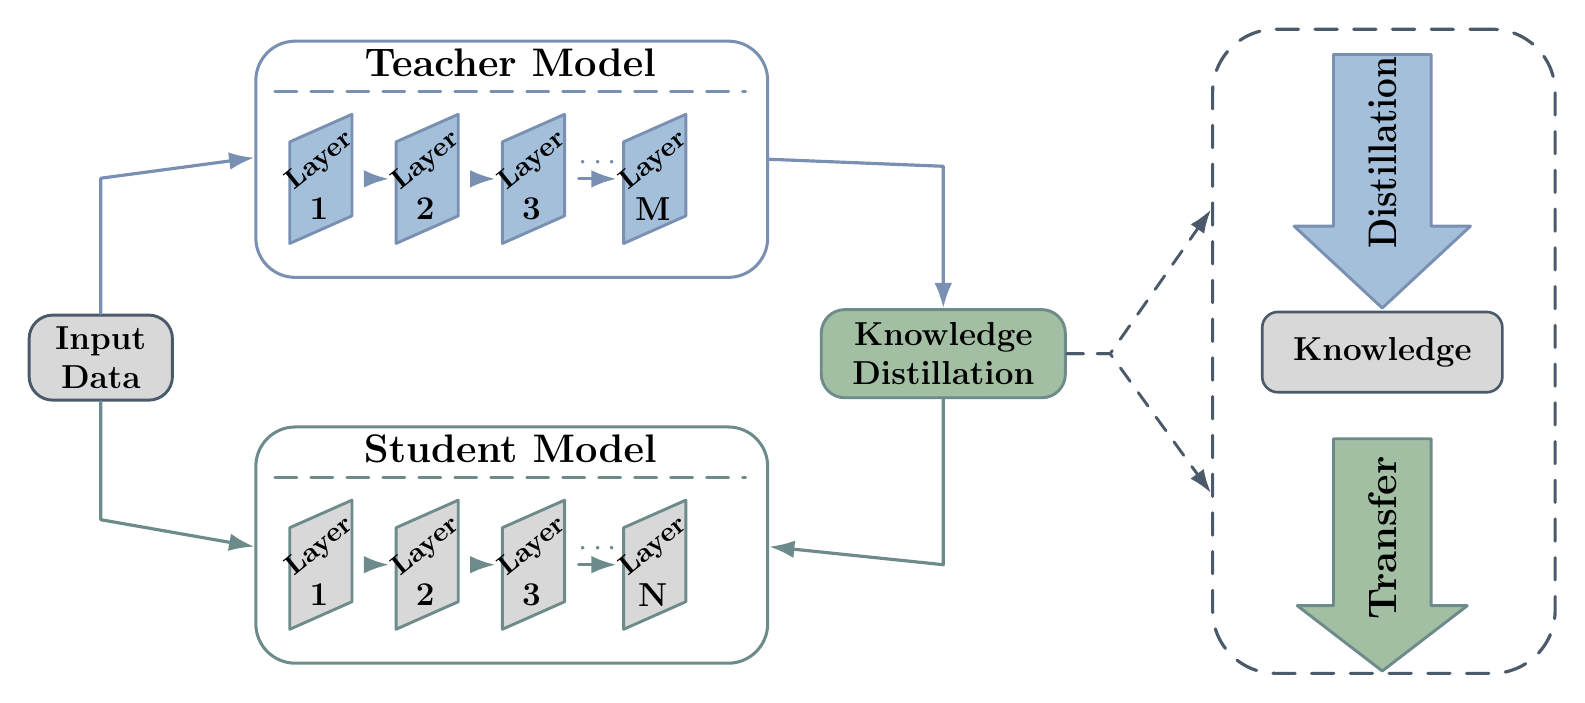
\begin{tikzpicture}[
  >=Latex,
  line cap=round,
  line join=round,
  font=\rmfamily,
  title/.style={font=\bfseries\Large, text=black, align=center},
  label/.style={font=\bfseries\large, text=black, align=center},
  smalllabel/.style={font=\bfseries\normalsize, text=black, align=center},
  arrowblue/.style={-{Latex[length=3.2mm,width=2.25mm]}, line width=1.15pt, draw=slateblue},
  arrowteal/.style={-{Latex[length=3.2mm,width=2.25mm]}, line width=1.15pt, draw=dustyteal},
  arrowgray/.style={-{Latex[length=3.0mm,width=2.1mm]}, line width=1.05pt, draw=deepmutedblue, dashed, dash pattern=on 6pt off 5pt}
]

% -----------------------------------------------------------------------------
% Muted palette requested by the user.
% Only these named colors are used for graphical elements; text stays black.
% Canvas sizing check:
%   model right edge = 2.90 + 6.50 = 9.40
%   KD left edge     = 11.65 - 3.10/2 = 10.10
%   horizontal gap   = 10.10 - 9.40 = 0.70 cm
%   student top      = 0.65 + 3.00 = 3.65
%   KD bottom        = 4.60 - 1.12/2 = 4.04
%   vertical gap     = 4.04 - 3.65 = 0.39 cm
% So the KD block is centered between the models and cannot overlap the student.
% -----------------------------------------------------------------------------
\definecolor{mistyblue}{HTML}{A3BFD9}
\definecolor{slateblue}{HTML}{7A90B2}
\definecolor{sagegreen}{HTML}{A3BFA3}
\definecolor{dustyteal}{HTML}{6E8B8B}
\definecolor{softgray}{HTML}{D8D8D8}
\definecolor{deepmutedblue}{HTML}{4A5A6A}

% Main geometry
\pgfmathsetmacro{\teacherX}{2.90}
\pgfmathsetmacro{\teacherY}{5.55}
\pgfmathsetmacro{\studentX}{2.90}
\pgfmathsetmacro{\studentY}{0.65}
\pgfmathsetmacro{\modelW}{6.50}
\pgfmathsetmacro{\modelH}{3.00}
\pgfmathsetmacro{\kdX}{11.65}
\pgfmathsetmacro{\kdY}{4.60}
\pgfmathsetmacro{\kdW}{3.10}
\pgfmathsetmacro{\kdH}{1.12}
\pgfmathsetmacro{\panelX}{15.05}
\pgfmathsetmacro{\panelY}{0.52}
\pgfmathsetmacro{\panelW}{4.35}
\pgfmathsetmacro{\panelH}{8.18}

% Slanted neural layer block.
% #1 name, #2 x, #3 y, #4 fill, #5 draw, #6 number
\newcommand{\LayerBlock}[6]{%
  \begin{scope}[shift={(#2,#3)}]
    \coordinate (#1-west) at (-0.52,0.00);
    \coordinate (#1-east) at (0.54,0.00);
    \path[draw=#5, fill=#4, line width=1.05pt]
      (-0.43,-0.82) -- (0.36,-0.47) -- (0.36,0.82) -- (-0.43,0.47) -- cycle;
    \node[font=\bfseries\normalsize, rotate=39, text=black] at (-0.05,0.23) {Layer};
    \node[font=\bfseries\large, text=black] at (-0.06,-0.38) {#6};
  \end{scope}%
}

% -----------------------------------------------------------------------------
% Input
% -----------------------------------------------------------------------------
\node[draw=deepmutedblue, fill=softgray, rounded corners=3mm,
      line width=1.05pt, minimum width=1.82cm, minimum height=1.08cm,
      label] (input) at (0.95,4.55) {Input\\Data};

% -----------------------------------------------------------------------------
% Teacher model
% -----------------------------------------------------------------------------
\coordinate (Tsw) at (\teacherX,\teacherY);
\node[draw=slateblue, rounded corners=5mm, line width=1.10pt,
      minimum width=\modelW cm, minimum height=\modelH cm,
      anchor=south west, inner sep=0pt] (teacherBox) at (Tsw) {};
\node[title] at ($(Tsw)+(0.5*\modelW,2.74)$) {Teacher Model};
\draw[draw=slateblue, dashed, dash pattern=on 8pt off 5pt, line width=0.95pt]
  ($(Tsw)+(0.26,2.38)$) -- ($(Tsw)+(\modelW-0.26,2.38)$);

\LayerBlock{t1}{3.78}{6.82}{mistyblue}{slateblue}{1}
\LayerBlock{t2}{5.13}{6.82}{mistyblue}{slateblue}{2}
\LayerBlock{t3}{6.48}{6.82}{mistyblue}{slateblue}{3}
\LayerBlock{tM}{8.02}{6.82}{mistyblue}{slateblue}{M}
\draw[arrowblue] (t1-east) -- (t2-west);
\draw[arrowblue] (t2-east) -- (t3-west);
\draw[arrowblue] (t3-east) -- node[midway, above=-1pt, font=\bfseries\large, text=slateblue] {$\cdots$} (tM-west);

% -----------------------------------------------------------------------------
% Student model
% -----------------------------------------------------------------------------
\coordinate (Ssw) at (\studentX,\studentY);
\node[draw=dustyteal, rounded corners=5mm, line width=1.10pt,
      minimum width=\modelW cm, minimum height=\modelH cm,
      anchor=south west, inner sep=0pt] (studentBox) at (Ssw) {};
\node[title] at ($(Ssw)+(0.5*\modelW,2.74)$) {Student Model};
\draw[draw=dustyteal, dashed, dash pattern=on 8pt off 5pt, line width=0.95pt]
  ($(Ssw)+(0.26,2.38)$) -- ($(Ssw)+(\modelW-0.26,2.38)$);

\LayerBlock{s1}{3.78}{1.92}{softgray}{dustyteal}{1}
\LayerBlock{s2}{5.13}{1.92}{softgray}{dustyteal}{2}
\LayerBlock{s3}{6.48}{1.92}{softgray}{dustyteal}{3}
\LayerBlock{sN}{8.02}{1.92}{softgray}{dustyteal}{N}
\draw[arrowteal] (s1-east) -- (s2-west);
\draw[arrowteal] (s2-east) -- (s3-west);
\draw[arrowteal] (s3-east) -- node[midway, above=-1pt, font=\bfseries\large, text=dustyteal] {$\cdots$} (sN-west);

% -----------------------------------------------------------------------------
% Knowledge distillation block - moved right and centered vertically.
% -----------------------------------------------------------------------------
\node[draw=dustyteal, fill=sagegreen, rounded corners=3mm, line width=1.05pt,
      minimum width=\kdW cm, minimum height=\kdH cm,
      label] (kd) at (\kdX,\kdY) {Knowledge\\Distillation};

% -----------------------------------------------------------------------------
% Right explanation panel
% -----------------------------------------------------------------------------
\node[draw=deepmutedblue, dashed, dash pattern=on 8pt off 6pt,
      rounded corners=8mm, line width=1.15pt,
      minimum width=\panelW cm, minimum height=\panelH cm,
      anchor=south west, inner sep=0pt] (panel) at (\panelX,\panelY) {};

% Distillation arrow
\begin{scope}[shift={($(panel.south west)+(0.5*\panelW,6.58)$)}]
  \path[draw=slateblue, fill=mistyblue, line width=1.05pt]
    (-0.62,1.30) -- (0.62,1.30) -- (0.62,-0.88) -- (1.12,-0.88)
    -- (0.00,-1.92) -- (-1.12,-0.88) -- (-0.62,-0.88) -- cycle;
  % Text size kept unchanged; only the arrow body is slightly taller.
  \node[rotate=90, text=black] at (0.00,0.05) {\scalebox{0.88}[1.00]{\bfseries\Large Distillation}};
\end{scope}

% Knowledge box
\node[draw=deepmutedblue, fill=softgray, rounded corners=2mm, line width=0.95pt,
      minimum width=3.05cm, minimum height=1.02cm,
      label] (knowledge) at ($(panel.south west)+(0.5*\panelW,4.10)$) {Knowledge};

% Transfer arrow
\begin{scope}[shift={($(panel.south west)+(0.5*\panelW,1.70)$)}]
  \path[draw=dustyteal, fill=sagegreen, line width=1.05pt]
    (-0.62,1.30) -- (0.62,1.30) -- (0.62,-0.82) -- (1.08,-0.82)
    -- (0.00,-1.65) -- (-1.08,-0.82) -- (-0.62,-0.82) -- cycle;
  \node[rotate=90, font=\bfseries\Large, text=black] at (0.00,0.04) {Transfer};
\end{scope}

% -----------------------------------------------------------------------------
% Flow arrows
% -----------------------------------------------------------------------------
\draw[arrowblue]
  (input.north) -- ++(0,1.72) -- ($(teacherBox.west)+(0,0.02)$);

\draw[arrowteal]
  (input.south) -- ++(0,-1.50) -- ($(studentBox.west)+(0,-0.02)$);

\draw[arrowblue]
  (teacherBox.east) -- (\kdX,6.98) -- (kd.north);

\draw[arrowteal]
  (kd.south) -- (\kdX,1.92) -- ($(studentBox.east)+(0,-0.02)$);

\draw[arrowgray]
  (kd.east) -- ++(0.55,0) -- ($(panel.west)+(0,1.80)$);
\draw[arrowgray]
  (kd.east) -- ++(0.55,0) -- ($(panel.west)+(0,-1.80)$);

\end{tikzpicture}
\end{document}
